\problemname{Last Guess}
If you spent any amount of time on social media at the end of last year, you
are probably familiar with the word finding game \emph{Wordle}, in which you
need to find a five-letter English word using at most six guesses. After each
guess, the letters in that guess are marked in either green, yellow or black to
provide information about the hidden word:

\begin{itemize}
  \item Green indicates that the letter is in the hidden word and appears in
    the same position.
\end{itemize}

\begin{itemize}
  \item Yellow indicates that the letter is in the hidden word, but in a
    different position.
  \item Black indicates that the letter has no more occurrences in the hidden word.
  \item If a letter appears more than once in the guessed word, first all the
    green markings for that letter are placed. Then, from left to right in the
    guessed word, yellow markings are placed for each remaining occurrence of
    the letter in the hidden word. Finally, black markings are placed for any
    surplus of the letter in the guessed word. See Figure~\ref{fig:last-guess}
    for an example.
\end{itemize}

\begin{figure}[h]
	\centering
	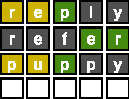
\includegraphics[width=0.30\textwidth]{sample}
	\caption{Illustration of Sample Input 1, where ``\texttt{upper}'' is
        the only valid last guess.}
	\label{fig:last-guess}
\end{figure}

In this problem, we consider a variant of Wordle where you need to find a
hidden word of length $\ell$ in at most $g$ guesses. Additionally, there is
\emph{no} requirement that the hidden word or any of the guesses are words of
any language; any string consisting of lowercase English letters is fine.

In your current play of this variant, you have already used all but one of your
guesses, and now you need to find the hidden word using your final guess. Find
any word that could be the hidden word based on the information you have.

\begin{Input}
  The input consists of:
  \begin{itemize}
    \item One line with two integers $g$ and $\ell$ ($2\le g\le 500$,
      $1\le \ell\le 500$), the maximal number of guesses allowed in the game and the length of
      the word.
    \item $g-1$ lines, each with two strings $s$ and $t$ of length $\ell$, where
      $s$ is one of the guesses so far and $t$ gives the colours for that guess
      according to the rules above. The string $s$ consists of lowercase English letters
		  (\texttt{a}-\texttt{z}) and the string $t$ consists of uppercase letters
		  `\texttt{G}', `\texttt{Y}', and `\texttt{B}' indicating green, yellow, and
          black respectively.
  \end{itemize}
  It is guaranteed that the input describes a valid state of a Wordle game
  before the last guess and that a valid solution exists, in the form of a
	length $\ell$ word consisting of lowercase English letters.
\end{Input}

\begin{Output}
  Output a valid last guess that gives you a chance of winning.

  If there are multiple valid solutions, you may output any one of them.
\end{Output}
